\documentclass[11pt]{article}
\usepackage[margin=1in]{geometry}
\usepackage{listings}
\usepackage{graphicx}
\usepackage{subfigure}
\usepackage{subcaption} % For subfigures
\usepackage{float} % for H option in figures
\usepackage{hyperref}
\usepackage[htt]{hyphenat} % for non-overflowing texttt
\usepackage{amsmath}

\usepackage{listings}

\title{Description of Source Data}
\author{Anton Zhitomirsky}

\usepackage{biblatex} %Imports biblatex package
\addbibresource{../../../source/bibliography.bib} %Import the bibliography file

\begin{document}

\maketitle

\tableofcontents

\section{Structure of source Data}

Results are structured in the file:

\begin{lstlisting}[language=bash]
/vol/biomedic3/bglocker/nnUNet
\end{lstlisting}

\begin{lstlisting}[language=inform]
-rwxr-xr-x   1 bglocker biomedia 236 Sep 24 15:16 exports
drwxr-sr-x   9 bglocker biomedia   9 Nov 25 10:55 nnUNet_preprocessed
drwxr-sr-x   9 bglocker biomedia  10 Nov 25 10:50 nnUNet_raw
drwxr-sr-x   9 bglocker biomedia   9 Nov 25 12:20 nnUNet_results
drwxr-sr-x  11 bglocker biomedia  11 Dec 16 09:10 nnUNet_testing
-rw-r--r--   1 bglocker biomedia 644 Oct 20 07:20 run_nnunet_0.sh
-rw-r--r--   1 bglocker biomedia 644 Oct 20 07:20 run_nnunet_1.sh
-rw-r--r--   1 bglocker biomedia 644 Oct 20 07:20 run_nnunet_2.sh
-rw-r--r--   1 bglocker biomedia 644 Oct 20 07:21 run_nnunet_3.sh
-rw-r--r--   1 bglocker biomedia 644 Oct 20 07:21 run_nnunet_4.sh
\end{lstlisting}

\subsection{nnUNet\_raw}\label{section:raw}

nnUNet\_raw has the original (training) images with manual annotations. Each Dataset below is treated as a binary segmentation problem. See Section\ref{section:itksnap}

\begin{lstlisting}[language=inform]
drwxr-sr-x  4 bglocker biomedia   5 Sep 17 13:47 Dataset001_Anorectum
drwxr-sr-x  3 bglocker biomedia   5 Sep 17 20:24 Dataset002_Bladder
drwxr-sr-x  3 bglocker biomedia   5 Sep 17 20:27 Dataset003_CTVn
drwxr-sr-x  3 bglocker biomedia   5 Sep 17 20:28 Dataset004_CTVp
drwxr-sr-x  3 bglocker biomedia   5 Sep 17 20:29 Dataset005_Parametrium
-rw-r--r--  1 bglocker biomedia 135 Nov 25 10:50 note
\end{lstlisting}

\subsection{nnUNet\_results}

The raw files from Section\ref{section:raw} are used to train an \href{https://github.com/MIC-DKFZ/nnUNet}{nnUNet model}. Which does a 5-fold cross validation, resulting in five models, each trained on 80 subjects and tested on 20 (there is a total of 100 subjects with manual annotations).

\subsubsection{Slurm script}

Each of the scripts are presented as bash scripts in \texttt{/vol/biomedic3/bglocker/nnUNet/run\_nnunet\_*.sh}. These are used to schedule the python program into the Slurm scheduler for running in the cloud.

\begin{lstlisting}[language=bash]
#!/bin/bash

# Example of running python script in a batch mode
#SBATCH -c 4                        # Number of CPU Cores
#SBATCH -p gpus                     # Partition (queue)
#SBATCH --gres gpu:1                # gpu:n, where n = number of GPUs
#SBATCH --mem 12288                 # memory pool for all cores
#SBATCH --nodelist lory          	# SLURM node
#SBATCH --output=slurm.%N.%j.log    # Standard output and error log

# Source virtual environment (pip)
source /vol/biomedic3/bglocker/coding/envs/nnunet/bin/activate

# Set env variables
source /vol/biomedic3/bglocker/nnUNet/exports

# Run python script
nnUNetv2_train 1 3d_fullres 4 # where 4 refers to which dataset we're 
                              # training
\end{lstlisting}

\begin{itemize}
    \item Source virtual environment
    
    This is activating the already created python environment. 

    \item Set env variables
    
    contains paths for raw, results and preprocessed directories

    \item Run python scripts 
    
    runs the script at \texttt{/vol/biomedic3/bglocker/coding/envs/nnunet}
\end{itemize}

\subsubsection{Python script}

No access

\subsection{nnUNet\_testing}

The models are then tested against 10 hold out manual semgentations with no manual segmentations.

\section{Viewing the Data}

\subsection{Itksnap}\label{section:itksnap}

The viewing tool used is ItkSnap, which was developed as an open source tool for viewing medical imaging scans. The view (Figure\ref{fig:view}) shows how you would see input data.

\begin{figure}[H]
    \centering
    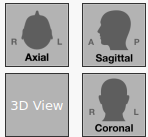
\includegraphics[]{images/view.png}
    \caption{view of all input data}\label{fig:view}
\end{figure}

With that we can use this tool to view input data. Here, the R and L stand for right and left respectively, and the A and P stand for Anterior and Posterior. We can provide a few other examples of viewing data displayed below in Figure\ref{fig:AnorectumImage}. We are further provided with manual annotation of the substructures. Figure\ref{fig:AnorectumLabel} shows an example of the annotation of the Anorectum. You can enable the 3D visual model through \texttt{Edit > 3D Panel > Toggle 3D view}.

\begin{figure}[H]
    \centering
    \captionsetup{width=0.45\textwidth}
    \begin{minipage}{.5\textwidth}
        \centering
        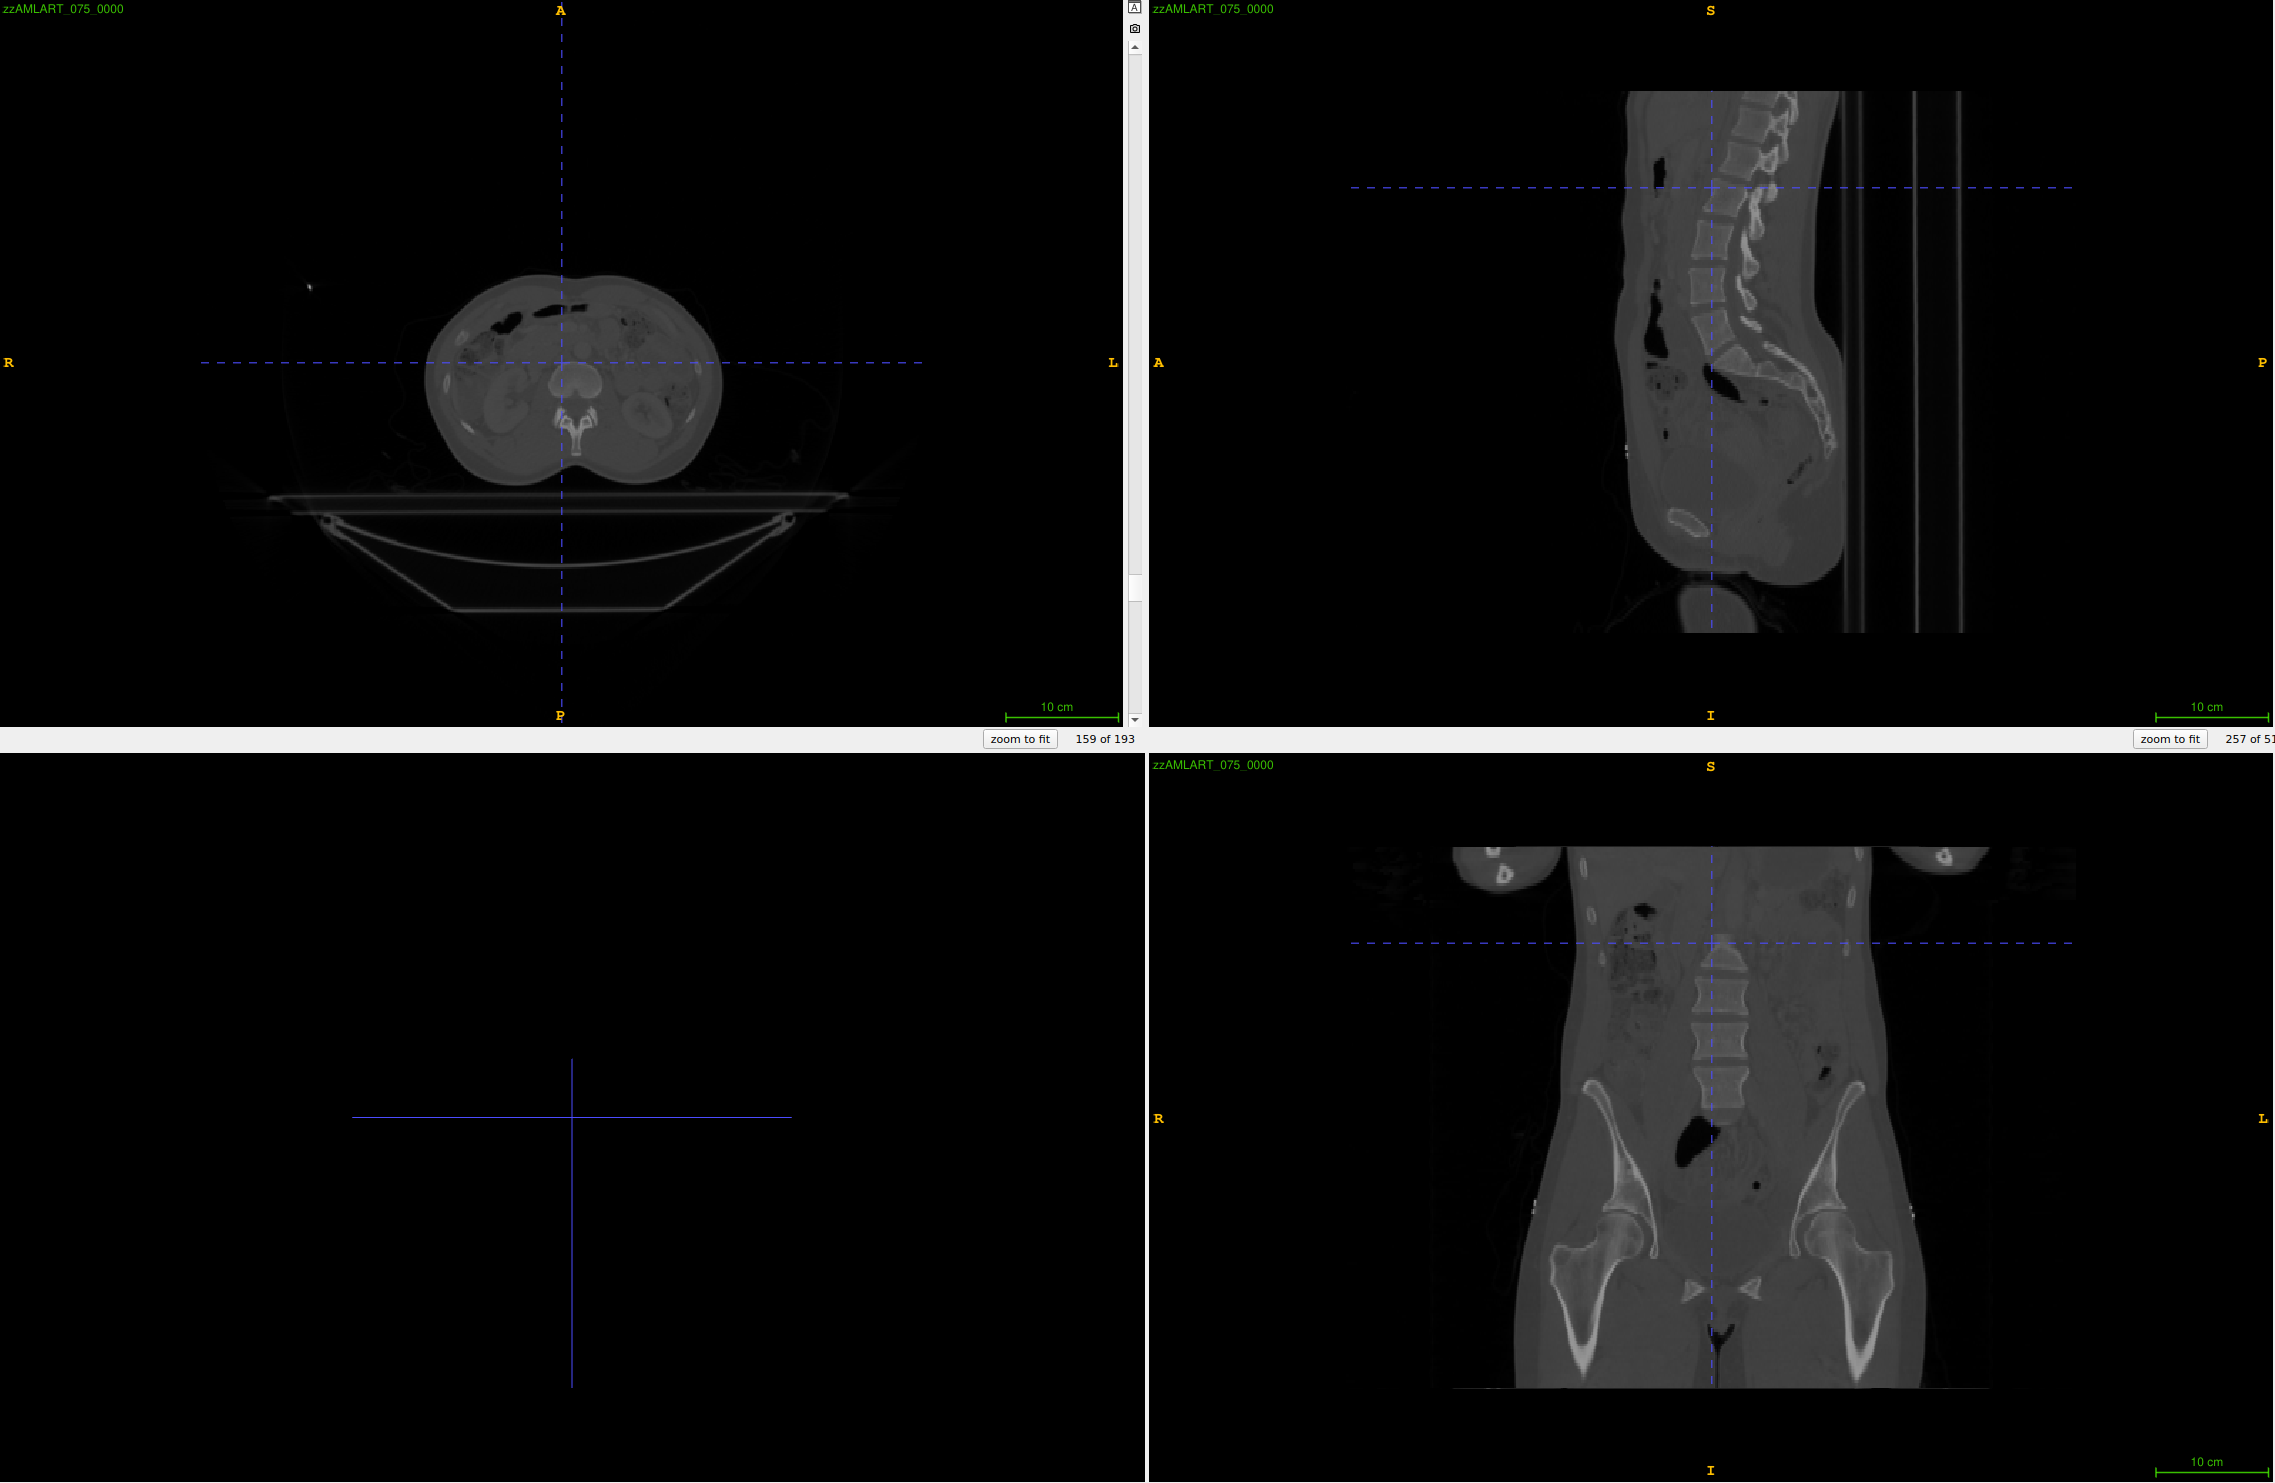
\includegraphics[width=\linewidth]{images/AnorectumImage.png}
        \caption{ItkSnap view of the Anorectum Raw Image}\label{fig:AnorectumImage}
    \end{minipage}%
    \begin{minipage}{.5\textwidth}
        \centering
        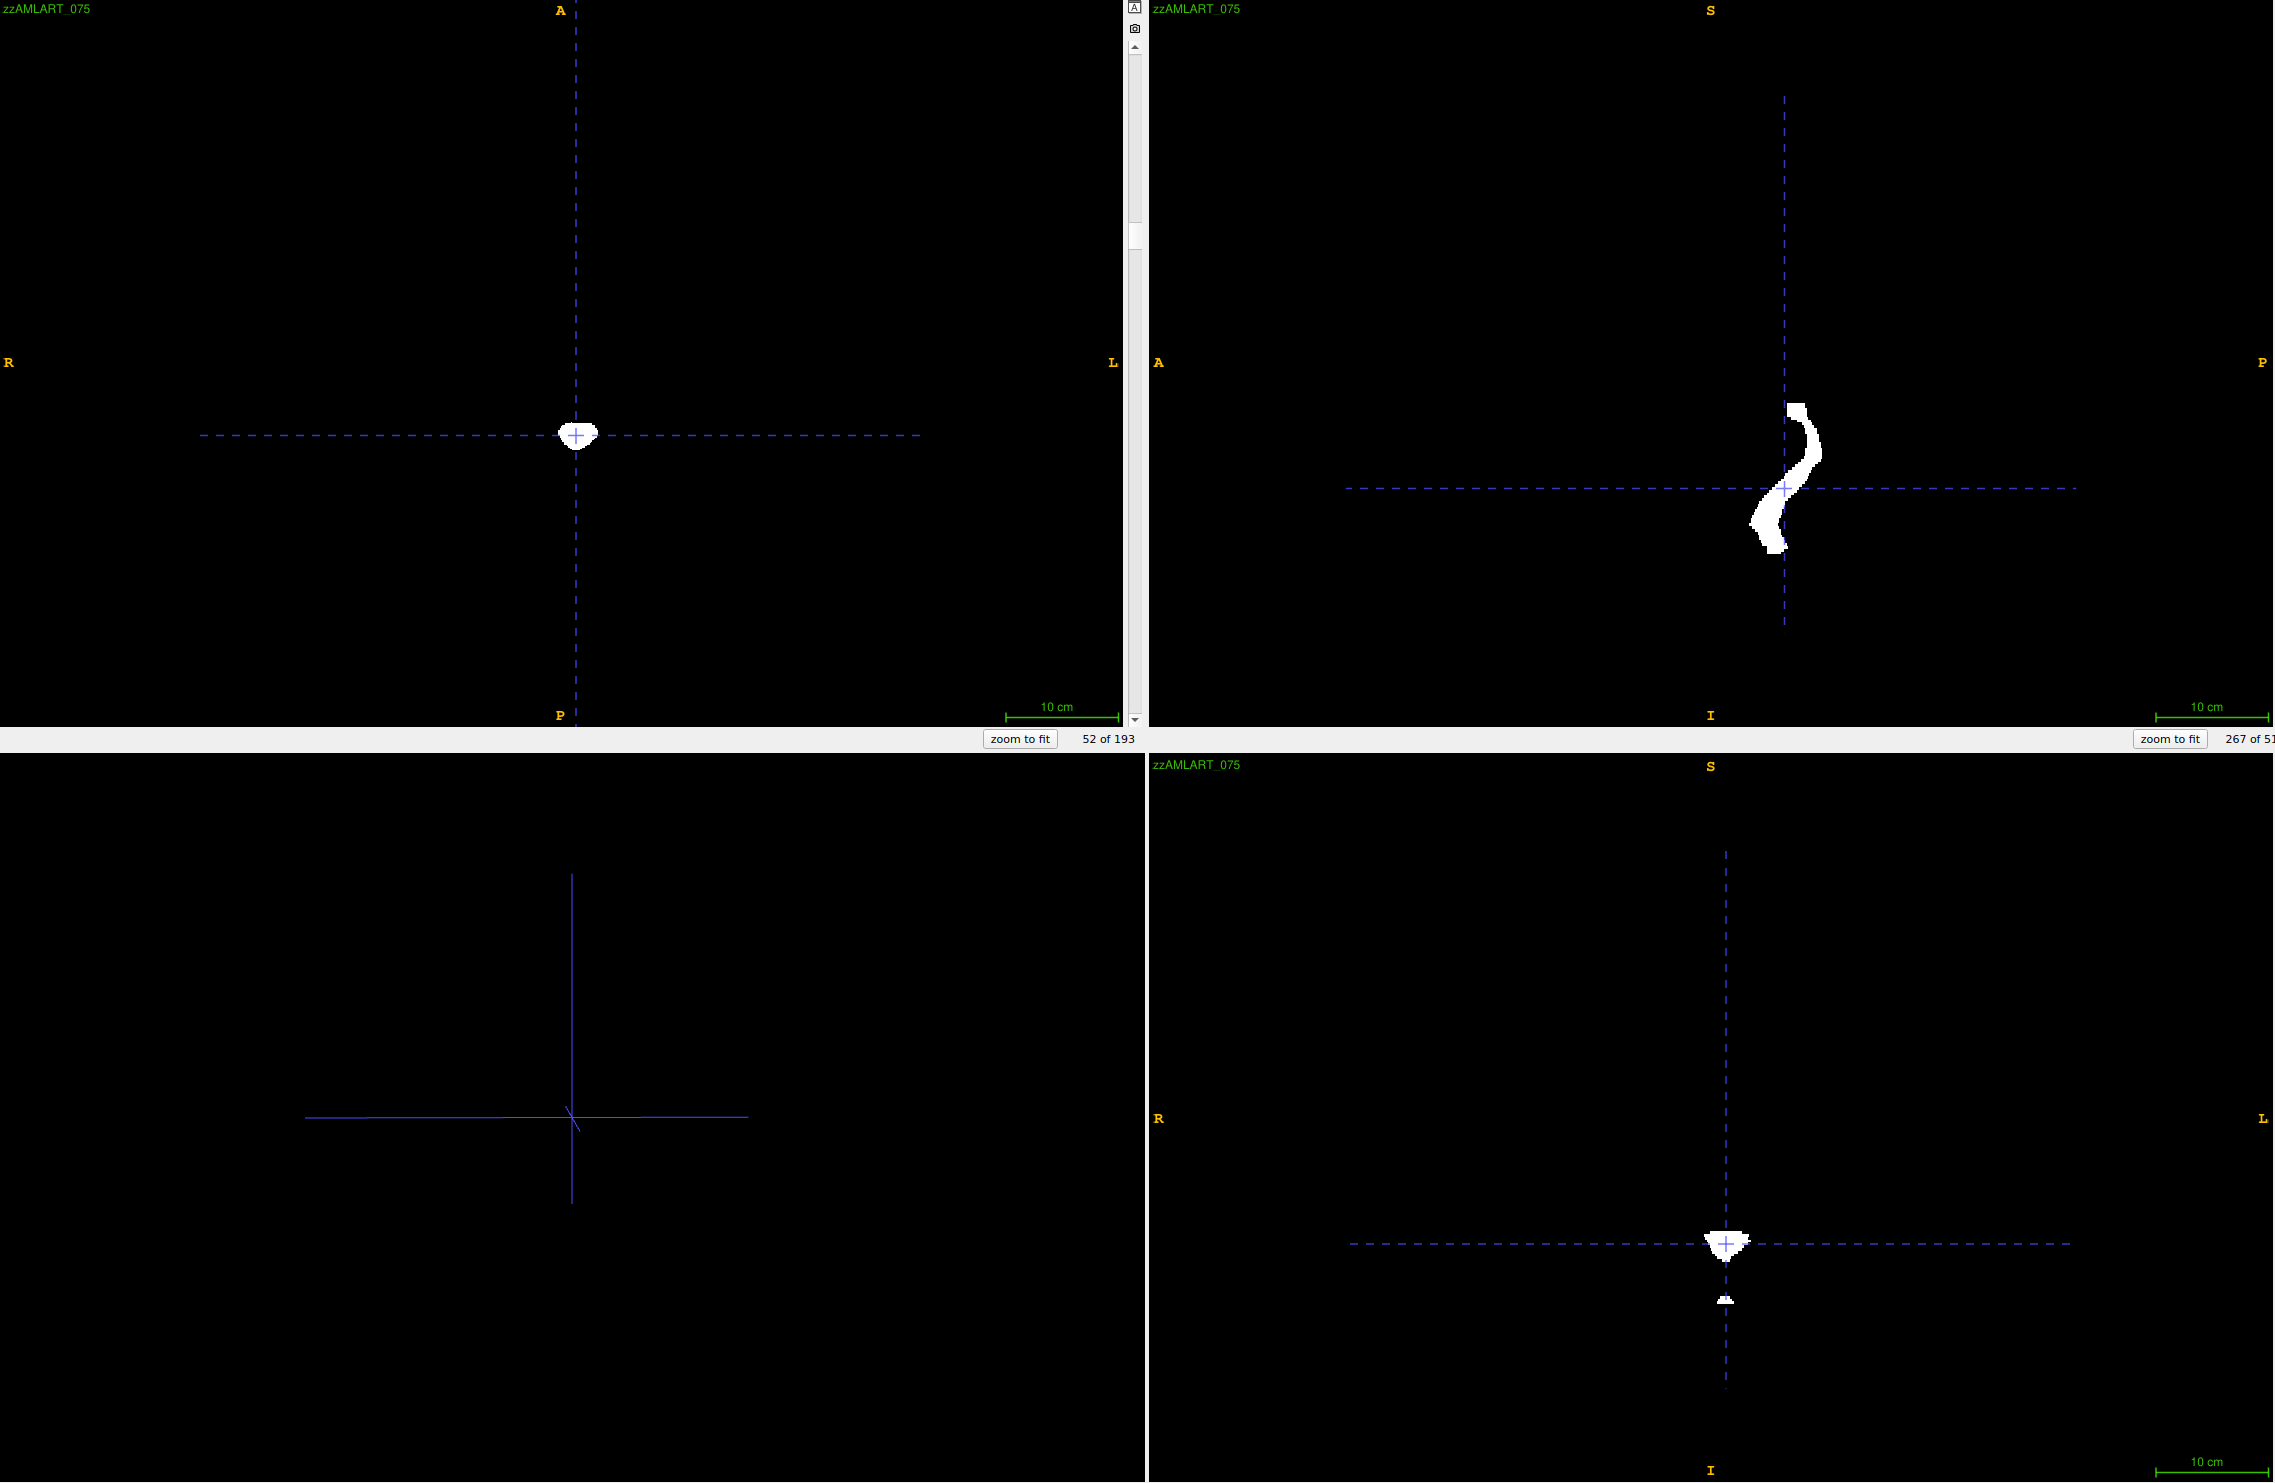
\includegraphics[width=\linewidth]{images/AnorectumLabel.png}
        \caption{ItkSnap view of the Anorectum Raw Image}\label{fig:AnorectumLabel}
    \end{minipage}%
\end{figure} 

\subsection{Reading the data in Python}

Please view the script at \texttt{research/source/code/performance/geometric/fetch-and-pre-process-data.py}

\section{NIfTI}

\subsection{What should a medical image contain as data?}

``A medical image is the representation of the internal structure
or function of an anatomic region in the form of an array of
picture elements called pixels or voxels. It is a discrete repre-
sentation resulting from a sampling/reconstruction process
that maps numerical values to positions of the space. The
number of pixels used to describe the field-of-view of a certain
acquisition modality is an expression of the detail with which
the anatomy or function can be depicted. What the numerical
value of the pixel expresses depends on the imaging modality,
the acquisition protocol, the reconstruction, and eventually,
the post-processing.'' \cite{file-formats}

\subsubsection{Components}

\begin{itemize}
    \item \textit{Pixel Depth}: ``number of bits used to encode the information of each pixel'' \cite{file-formats}
    \item \textit{Photometric Interpretation}:  ``specifies how the pixel data
    should be interpreted for the correct image display as a 
    monochrome or color image. To specify if color information is or is
    not stored in the image pixel values, we introduce the concept
    of samples per pixel (also known as number of channels).
    Monochrome images have one sample per pixel and no color
    information stored in the image. A scale of shades of gray
    from black to white is used to display the images. The number
    of shades of gray depends clearly from the number of bits used
    to store the sample that, in this case, coincide with the pixel
    depth'' \cite{file-formats}

    For our case, this will be grey scale 

    \item \textit{Metadata}: information that describe the image
    \item \textit{Pixel Data}: the section where the numerical values of the pixels are stored
\end{itemize}

\subsection{NIfTI file format}

The files are stored in a \texttt{.nii} format. This is a NIfTI file format which has had more prominence than the dicom file format recently \cite{dicom-to-nifti-conversion}. 

\begin{itemize}
    \item ``NIfTI is simple and easy to support''
    \item ``Neuroimaging Informatics Technology Initiativ''\cite{file-formats}
    \item ``allows spatial orientation information to be stored more fully''\cite{dicom-to-nifti-conversion}. Therefore, NIfTI-compliant software should reduce the chance of making ``left–right ambiguity''\cite{file-formats,dicom-to-nifti-conversion}
\end{itemize}

\begin{figure}[H]
    \centering
    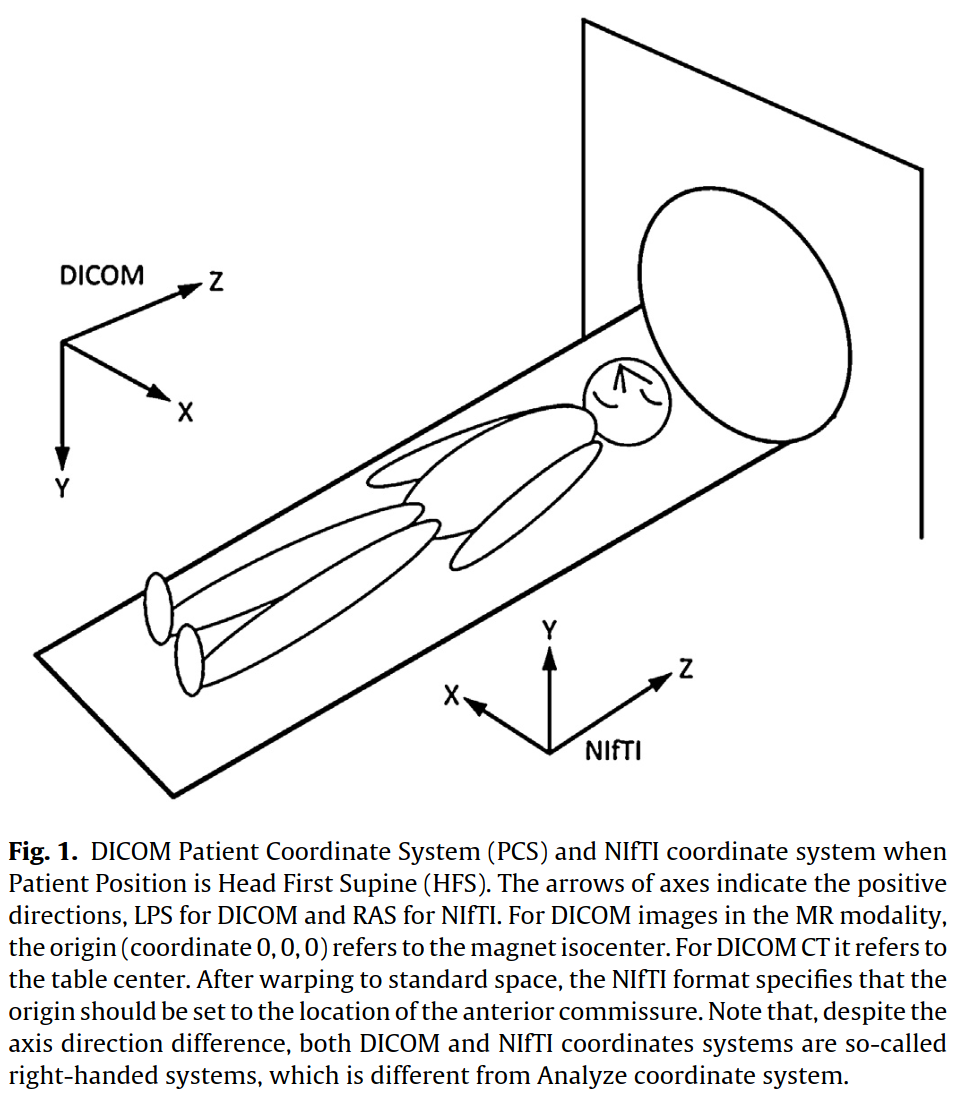
\includegraphics[width=.75\linewidth]{images/dicom-nifti.png}
    \caption{taken from \cite{dicom-to-nifti-conversion}}
\end{figure}

\subsection{Header File}

One may observe the header of the file:

\begin{lstlisting}[language=python]
{
    'ITK_FileNotes': ''
    'ITK_original_direction': '[UNKNOWN_PRINT_CHARACTERISTICS]\n'
    'ITK_original_spacing': '[UNKNOWN_PRINT_CHARACTERISTICS]\n'
    'aux_file': ''
    'bitpix': '32'
    'cal_max': '0'
    'cal_min': '0'
    'datatype': '8'
    'descrip': ''
    'dim[0]': '3'
    'dim[1]': '512'
    'dim[2]': '512'
    'dim[3]': '193'
    'dim[4]': '1'
    'dim[5]': '1'
    'dim[6]': '1'
    'dim[7]': '1'
    'dim_info': '0'
    'intent_code': '0'
    'intent_name': ''
    'intent_p1': '0'
    'intent_p2': '0'
    'intent_p3': '0'
    'nifti_type': '1'
    'pixdim[0]': '0'
    'pixdim[1]': '1.26953'
    'pixdim[2]': '1.26953'
    'pixdim[3]': '2.5'
    'pixdim[4]': '0'
    'pixdim[5]': '0'
    'pixdim[6]': '0'
    'pixdim[7]': '0'
    'qfac': '[UNKNOWN_PRINT_CHARACTERISTICS]\n'
    'qform_code': '1'
    'qform_code_name': 'NIFTI_XFORM_SCANNER_ANAT'
    'qoffset_x': '325'
    'qoffset_y': '325'
    'qoffset_z': '-155'
    'qto_xyz': '[UNKNOWN_PRINT_CHARACTERISTICS]\n'
    'quatern_b': '0'
    'quatern_c': '0'
    'quatern_d': '1'
    'scl_inter': '0'
    'scl_slope': '1'
    'sform_code': '1'
    'sform_code_name': 'NIFTI_XFORM_SCANNER_ANAT'
    'slice_code': '0'
    'slice_duration': '0'
    'slice_end': '0'
    'slice_start': '0'
    'srow_x': '-1.26953 0 0 325'
    'srow_y': '0 -1.26953 0 325'
    'srow_z': '0 0 2.5 -155'
    'toffset': '0'
    'vox_offset': '352'
    'xyzt_units': '2'
}
\end{lstlisting}

\begin{figure}[H]
    \centering
    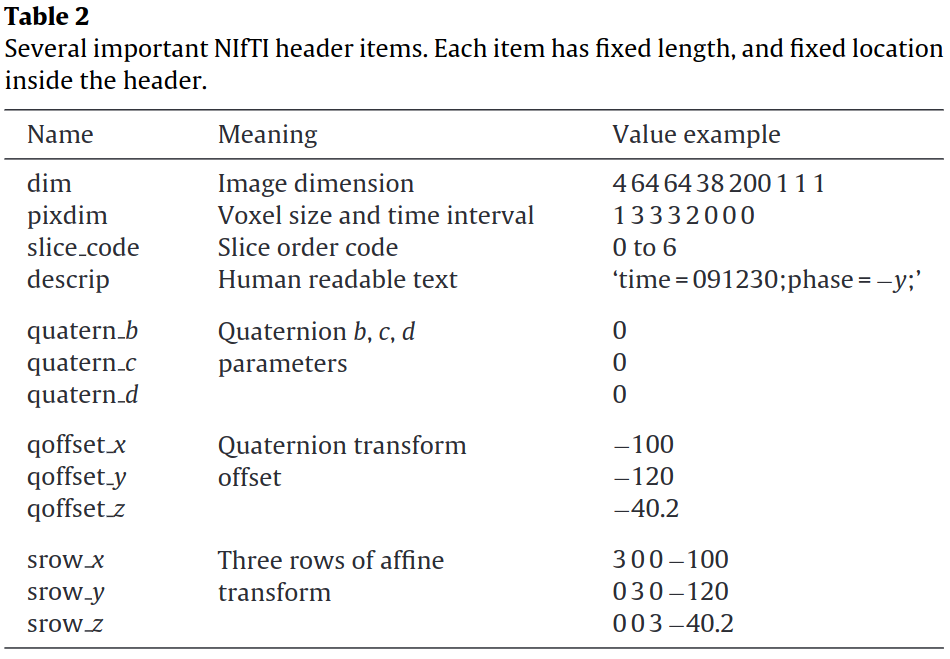
\includegraphics[width=.75\linewidth]{images/header-info.png}
    \caption{taken from \cite{dicom-to-nifti-conversion} with further information available from \cite{nifti-headers}}
\end{figure}

\subsubsection{Dimension}

Starting indexing at 0, we have: 

\begin{equation*}
    dim = \begin{bmatrix}3 \\ 512 \\ 512 \\ 193 \\ 1 \\ 1 \\ 1 \\ 1\end{bmatrix}
\end{equation*}


From Page 3 of \cite{nifti-data-format} 

\begin{itemize}
    \item dim[3] $\neq$ 1, therefore this is not a single slice. Instead, dim[3] $>$ 1, so there is several slices.
    \item dim[5] $=$ 1, therefore, this is a statistical parameter stored in \texttt{intent\_p1/2/3}. These are all set to 0, therefore, this is a null dimension.
\end{itemize}

\subsubsection{PixDim}

BitPix (32) is the ``number of bits per voxel [...], which MUST correspond with the datatype field'' \cite{nifti-headers}. PixDim is the grid spacing \cite{nifti-headers}. We indicate the units of pixdim with ``char xyzt\_units'' \cite{nifti-headers} which is 2 in our case. We have no temporal dimension because ``dimensions 1,2,3 are for x,y,z; dimension 4 is for time (t)'' \cite{nifti-headers}. A value of 2 means ``\#define NIFTI\_UNITS\_MM      2'' \cite{nifti-headers} where bits 0 .. 2 specify the units of our dimensions, so $2 \equiv 010_2$ hence we measure our dimensions in mm.

\subsubsection{The Rest}

The rest are not relevant to our cause - the library supposedly does everything else for us.

\subsection{What do the pixels values mean in NIfTI}

\subsubsection{ImagesTr}

When you read in the data for the \texttt{.nii} then you get a list of 2658 unique values. This is not as simple as binary segmentation task of 0s and 1s, we have negatives from -1000 to positives up to 3140. Yeah duh, I mistakenly was analyzing the raw input which will have variable pixel strengths depending on the part of the body it is displaying.

\subsubsection{LabelsTr}

\begin{lstlisting}[language=python]
>>> values, count = fetch.np.unique(itk_image, return_counts=True)
>>> values
array([0, 1], dtype=uint8)
>>> count
array([50579427,    14365])
\end{lstlisting}

\section{What is CT}

from \href{https://www.nhs.uk/conditions/ct-scan/}{NHS}

\begin{itemize}
    \item ``A CT scan is a test that takes detailed pictures of the inside of your body. It's usually used to diagnose conditions or check how well treatment is working''.
\end{itemize}

from \cite{ct-scan}

\begin{itemize}
    \item ``The CT scan is essentially an X-ray study, where a series of rays are rotated around a specified body part, and computer-generated cross-sectional images are produced. The advantage of these tomographic images compared to conventional X-rays is that they contain detailed information of a specified area in cross-section, eliminating the superimposition of images, which provides a tremendous advantage over plain films. ''
    \item The CT scanner machine rotates the X-ray tube around the patient's body through a circular structure known as the gantry. Each time the machine rotates, computerized information is acquired. The patient is slowly moved up or down in the table, and different cross-section images are produced. In each rotation, a 2D image slice is constructed. Each subsequent image slice's thickness is decided on the operator and the physician/radiologist's request but usually ranges from 1 to 10 millimeters. The gantry can be moved at the desired angle to accommodate the best cross-sectional image. When the desired number of slices are obtained, a scan is reproduced into the computer image and can easily be reproduced and stored.
    \item 
\end{itemize}

\printbibliography


\end{document}